\documentclass[PhD]{iitmdiss}
\usepackage{times}
\usepackage{t1enc}

%\usepackage[dvips]{graphicx}
%\usepackage[hypertex]{hyperref} % hyperlinks for references.
\usepackage{hyperref} % hyperlinks for references.
\usepackage{amsmath} % easier math formulae, align, subequations \ldots
\usepackage{graphicx}
\usepackage{epstopdf}

\usepackage{macros}

\title{Gate sizing for energy efficient and secure digital designs.}

\author{Patanjali SLPSK}

\date{December 2018}
\department{COMPUTER SCIENCE AND ENGINEERING}


\begin{document}

%\nocite{*}
\maketitle

 \newpage
\
\thispagestyle{empty}
\clearpage

% The main text will follow from this point so set the page numbering
% to arabic from here on.
\pagenumbering{arabic}
\setcounter{page}{1}

%\afterpage{\null\newpage}


\section{Introduction}
\label{synopsis:intro}
\input{synopsis/intro1}

\section{Motivation}
\label{synopsis:motivation}
\section{Motivation for Integrating Security requirements into an EDA Flow}
\label{sec:motivation}

%In this section, we provide a concrete example that highlights the fact that existing EDA optimizations indeed have an effect on the security of the device. 
%need for a security-aware EDA flow that optimizes security along with the typical requirements. We take an AES-128 design and synthesize it to generate six different netlists each of which is optimized to meet a different objective such as low power, high performance \& smaller area, low power \& smaller area, and high performance \& low power. % as shown in Table~\ref{tab:design}. 
%The design configurations with their area, delay, and power numbers are shown in Table~\ref{tab:design}. We then analyze the side-channel resistance of each netlist using the Mean Traces to Leak (MTL) metric defined in Section~\ref{}. %The number of power traces needed to guess the key, called mean time for disclosure (MTD), is shown in the fourth column of Table~\ref{tab:design}. A higher MTD value indicates that the attacker needs to collect large number of samples in order to guess the AES key and a smaller MTD value indicates that the device can be easily exploited via the power side-channel.

% \todo[inline]{table 1 hardly makes sense! out of 6 designs on the 3rd one actually serves the purpose.}
\begin{table}[t!]
\scriptsize
\centering

\caption{Impact of design requirements on Area, Power, Delay and the magnitude of TVLA score at the end of 4000 traces for an AES design.  }
\begin{tabular}{|c|c|c|c|c|c|}

\hline

\textbf{\begin{tabular}[c]{@{}c@{}}Design \\ Choices\end{tabular}} & \textbf{Area} & \textbf{\begin{tabular}[c]{@{}c@{}}Delay \\ (ns)\end{tabular}} & \textbf{\begin{tabular}[c]{@{}c@{}}Static\\  Power ($\mu W$)\end{tabular}} & \textbf{TVLA}\\ \hline
I -- Area $\downarrow$ Power $\downarrow$ &       78883        &                  0.48                                              &                            492.4                                  & 11.077                                                                          \\ \hline
II  -- Area $\downarrow$        &        58439       &                 0.48                                               &    602.42             &  11.41                                                                                                            \\ \hline
III -- Area $\downarrow$ Delay $\downarrow$      &       82545        &               0.47                                                 &    513.40               & 8.22  \\ \hline
IV -- Power $\downarrow$ Delay $\downarrow$     &     102256          &             0.47                                                   &               683.41     & 10.65 \\ \hline
V --    Power $\downarrow$ &    79097           &             0.48                                                   &     482.80              &   9.95\\ \hline
VI -- Delay $\downarrow$    &        91822       &        0.32                                                        &     2105.8                  &  13.97       

\\ \hline

\end{tabular}
\label{tab:design}
\end{table}
\begin{figure}[t!]
\centering
  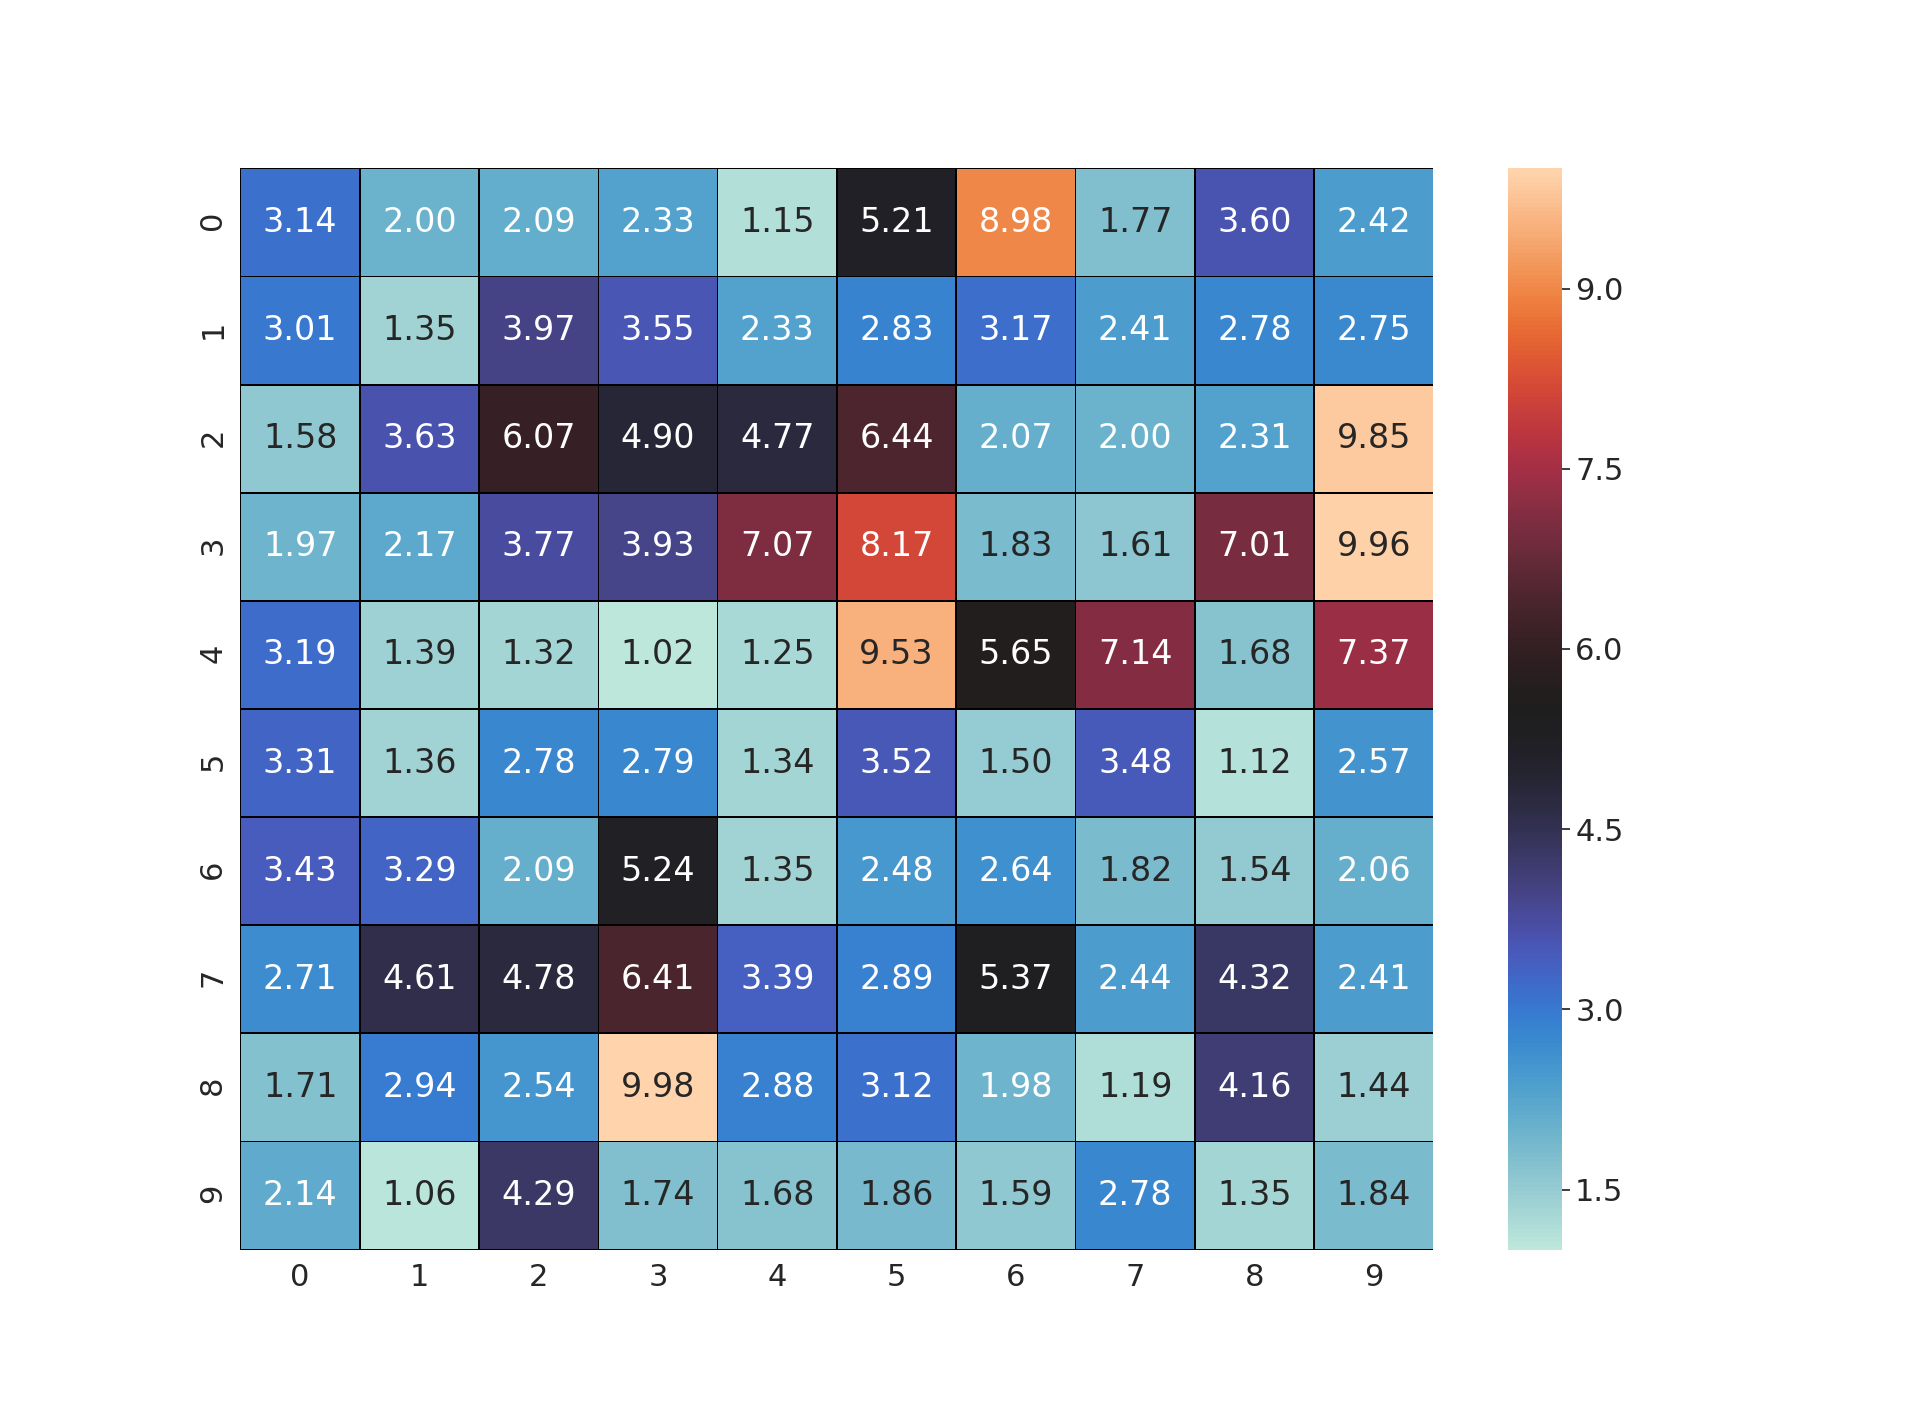
\includegraphics[scale=0.20]{Chapter4/fig/aes_before.png}  
\caption{The TVLA profile of the AES design, with the design divided into a $10\times 10$ grid and the TVLA score of each cell calculated independently. Of the 100 cells, 21 have a TVLA score greater than 4.5. The overall TVLA score of the netlist is 8.22. }
\label{fig:aesopt}
\end{figure}

In this section, we use three critical observations to motivate the use of EDA tools to achieve side-channel security.

\begin{namedthm}{Observation}
EDA algorithms influence the side-channel security of a design.
\end{namedthm}

{\flushleft We} synthesized an AES cipher to meet various design objectives. Table~\ref{tab:design} shows the area, delay, power, and security (TVLA score) of six (I to VI) different netlists. Each netlist was synthesized using the same AES design and used the same EDA tool (Synopsis Design Compiler). The EDA tool was configured with different design requirements for each synthesis. For example, netlist II was synthesized with the objective to reduce area, while netlist IV was synthesized to reduce both power and delay.
For each design, we computed the TVLA score from 4000 pairs of simulated power traces. As seen in the table, we obtain different TVLA scores for each netlist. We thus conclude that design requirements used by an EDA tool have an impact on the overall security of the final device. This experiment corroborates the observations made in~\cite{Verbauwhede:2005, danger:2017, yang:2005}. 
\begin{figure}[t!]
\centering
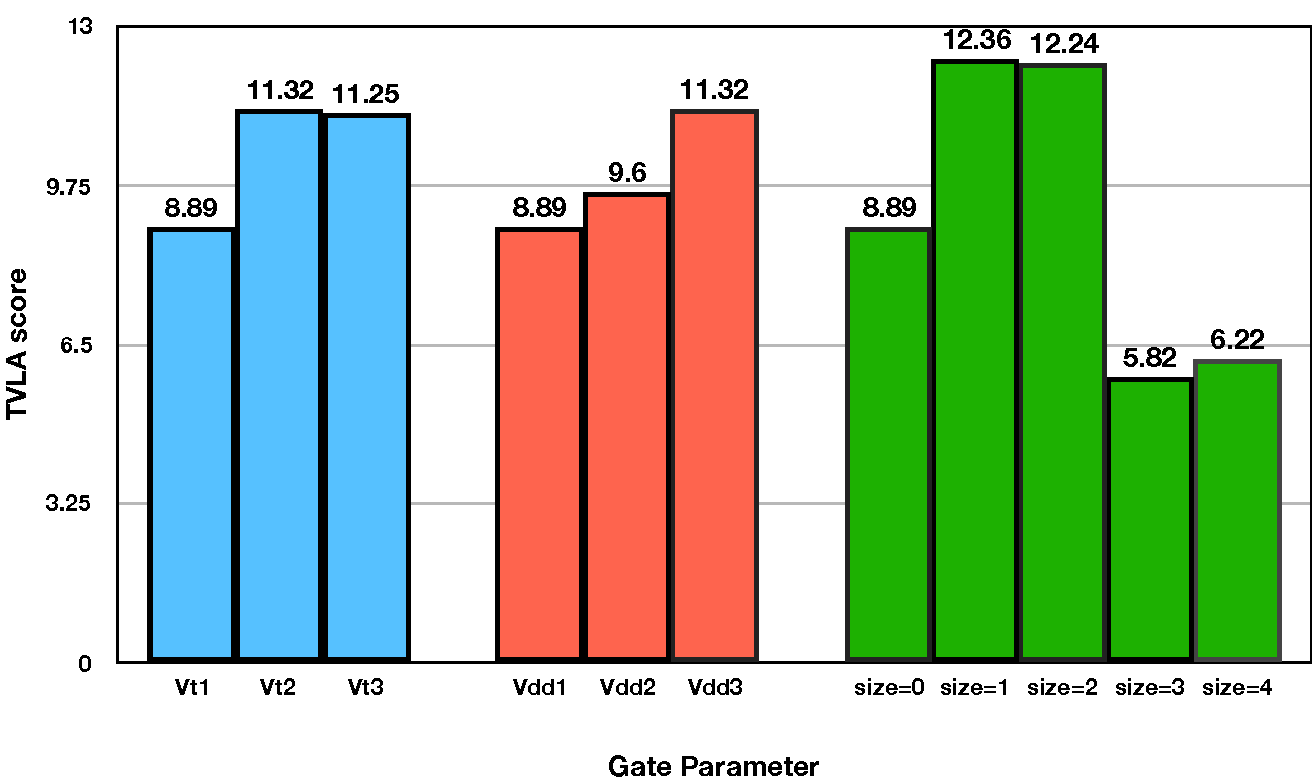
\includegraphics[scale=0.35]{Chapter4/fig/tvla_gate.pdf}
\caption{Variation of TVLA score with $V_{t}$,$V_{dd}$ and $size$ for an AND tree design.}
\label{fig:gateparam}
%\vspace{-15pt}
\end{figure}


% \begin{figure*}[ht!]
% \centering
% \begin{subfigure}{.5\textwidth}
%   \centering
%   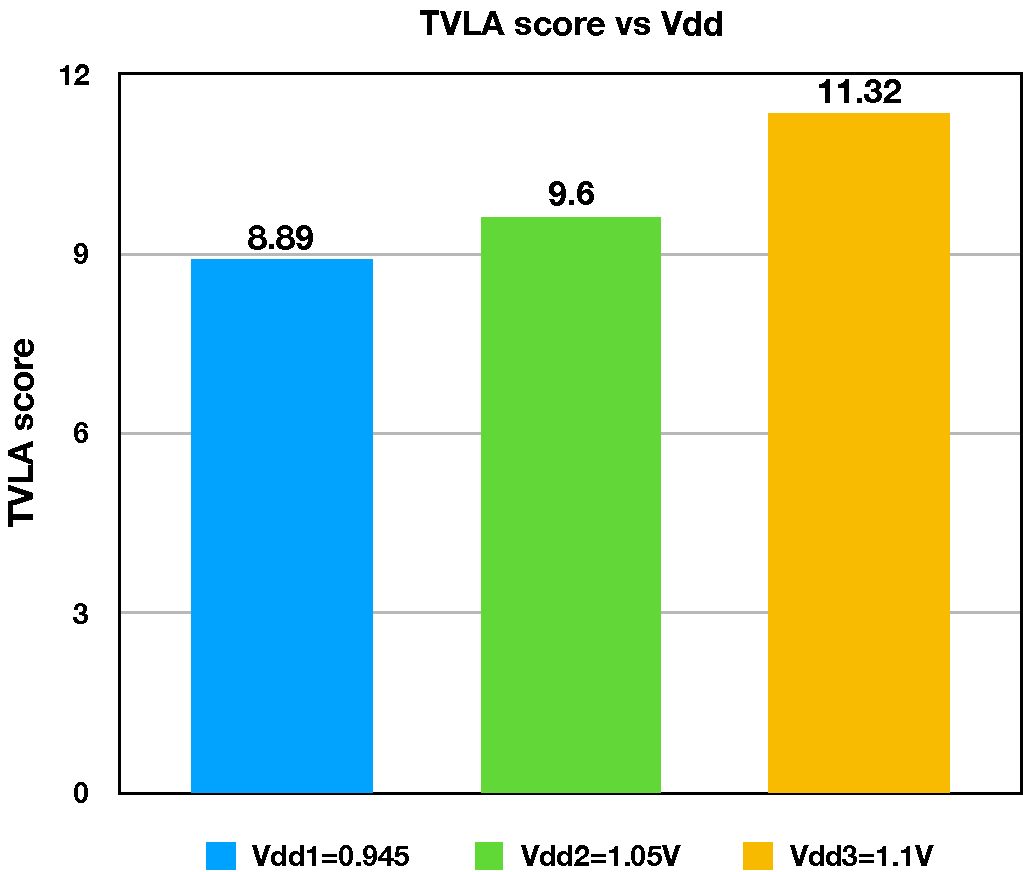
\includegraphics[width=10cm,height=5cm,keepaspectratio]{fig/tvla_vdd.pdf}
%   \caption{Variation of TVLA score with $V_{dd}$.}
%   \label{fig:sub1}
% \end{subfigure}%
% \begin{subfigure}{.55\textwidth}
%   \centering
%   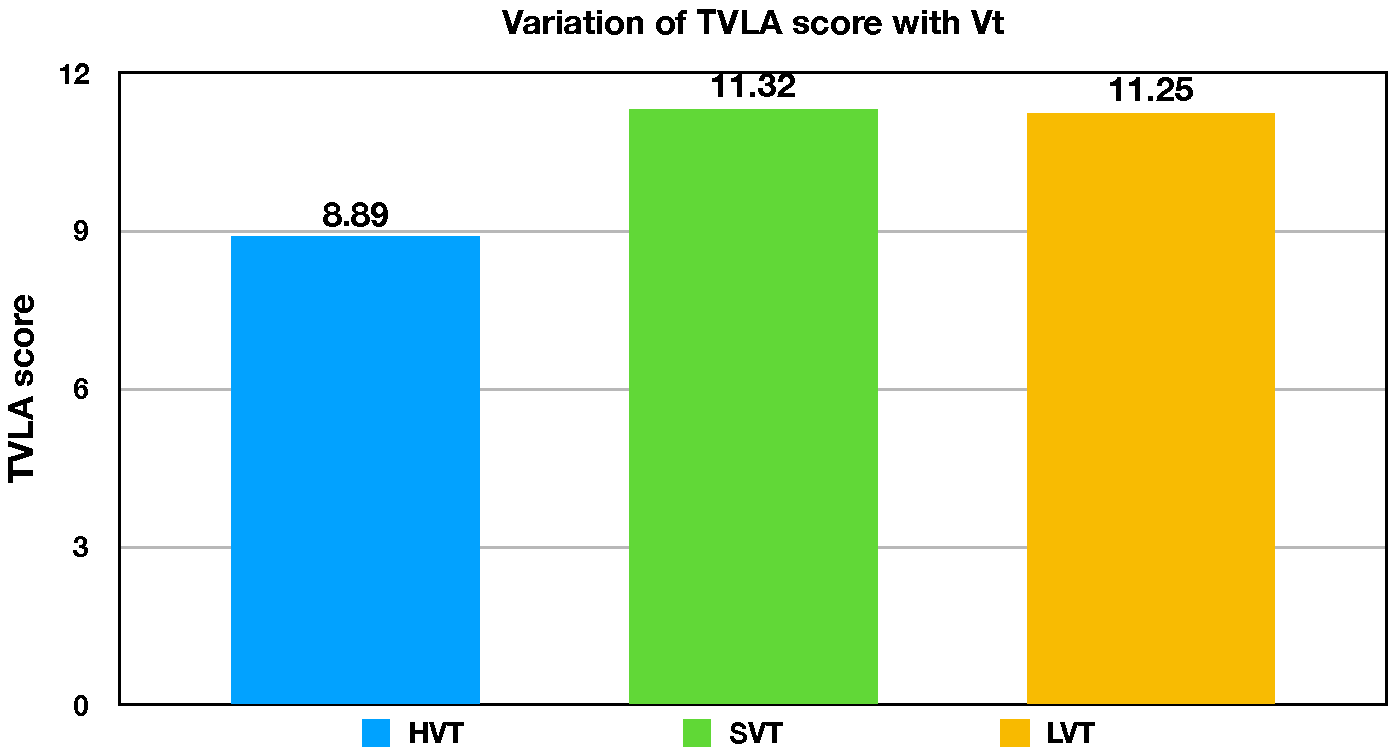
\includegraphics[width=8cm,height=5cm,keepaspectratio]{fig/tvla_vt.pdf}
%   \caption{Variation of TVLA score with $V_{t}$. }
%   \label{fig:sub2}
% \end{subfigure}
% \begin{subfigure}{.75\textwidth}
%   \centering
%   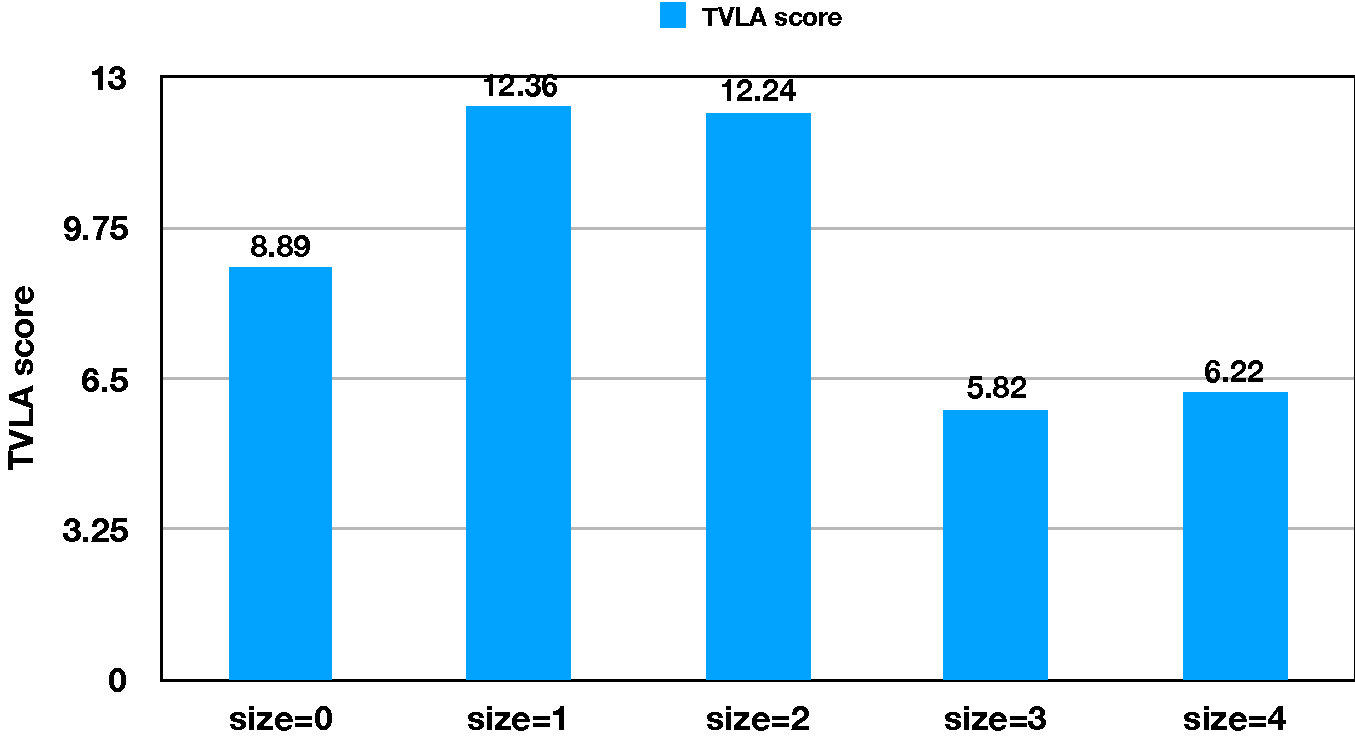
\includegraphics[width=8cm,height=5cm,keepaspectratio]{fig/tvla_size.pdf}
%   \caption{Variation of TVLA score with size. }
%   \label{fig:sub3}
% \end{subfigure}
% % \begin{subfigure}{.75\textwidth}
% %   \centering
% %   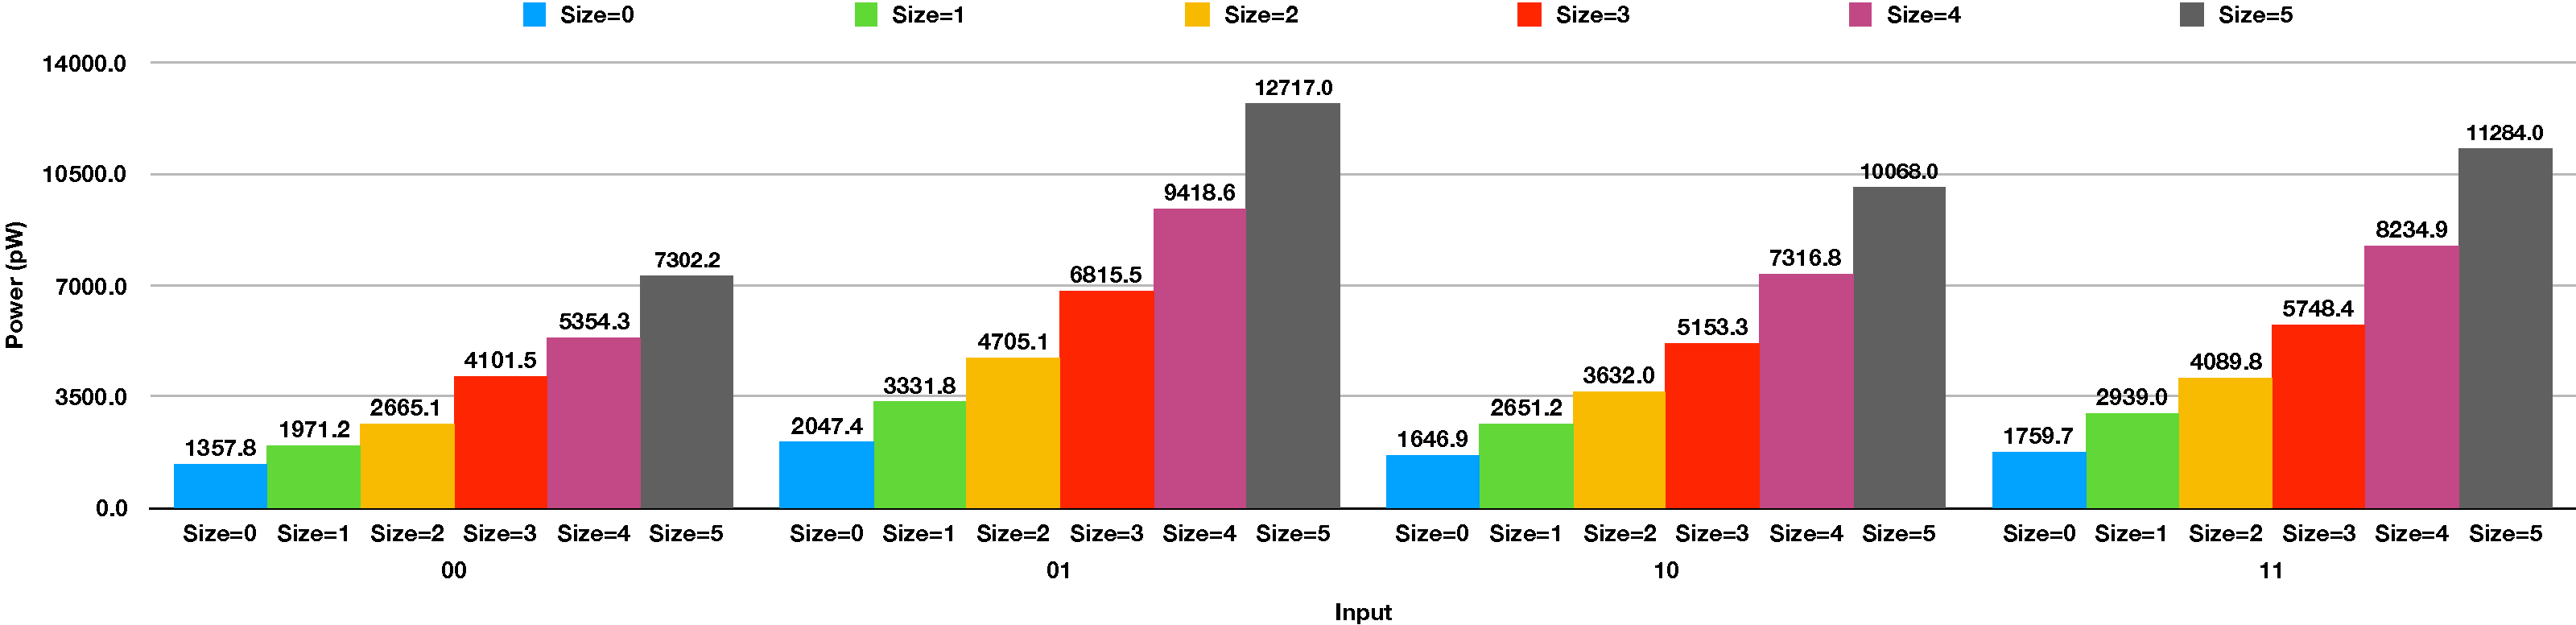
\includegraphics[width=14cm,height=5cm]{fig/sizevsinput.pdf}
% %   \caption{Variation of dynamic power of an AND gate with $size$ and logic level}
% %   \label{fig:sub3}
% % \end{subfigure}%
% % \caption{Figure showing variation of dynamic power of an AND gate with $V_{dd}$, $V_{t}$ and $size$.}
% \label{fig:power}
% \end{figure*}

% \begin{figure*}[ht!]
% \centering
% \begin{subfigure}{.5\textwidth}
%   \centering
%   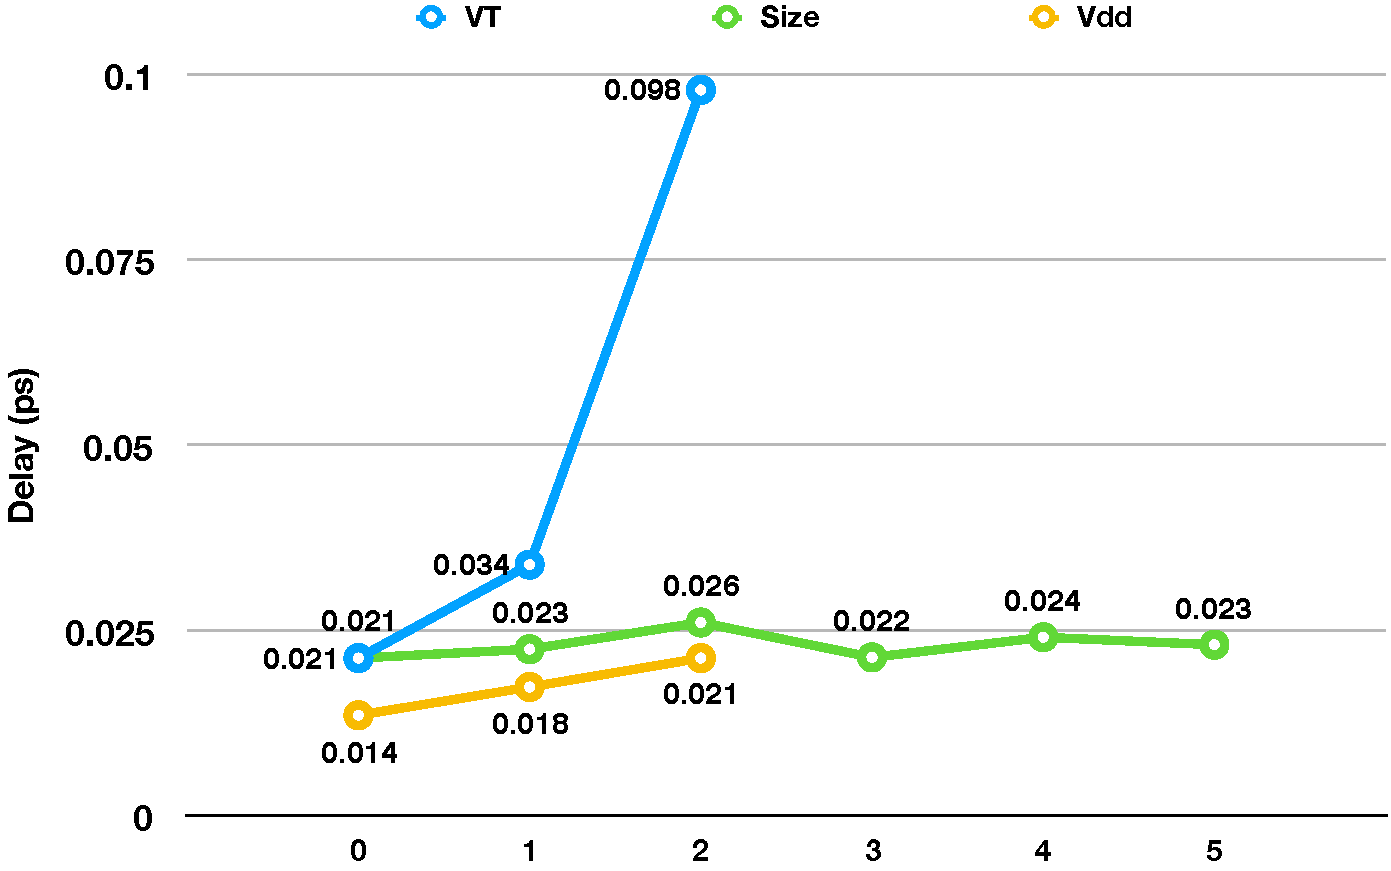
\includegraphics[width=10cm,height=5cm]{fig/delayvariation.pdf}
%   \caption{Variation of delay of an AND gate with $V_{dd}$,$V_{t}$ and $size$.}
%   \label{fig:delay1}
% \end{subfigure}%
% \begin{subfigure}{.55\textwidth}
%   \centering
%   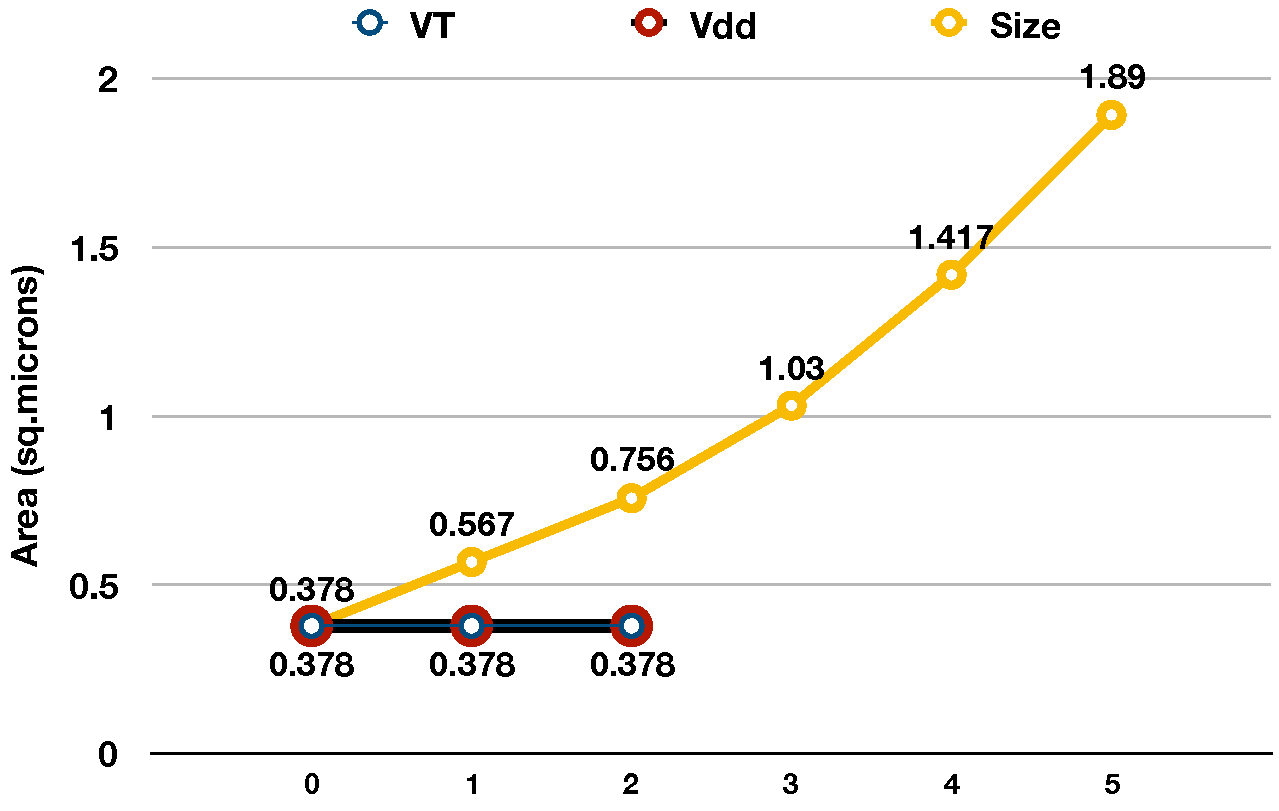
\includegraphics[width=8cm,height=5cm]{fig/areavariation.pdf}
%   \caption{Variation of area of an AND gate with $V_{dd}$, $V_{t}$ and $size$. }
%   \label{fig:delay2}
% \end{subfigure}
% \caption{Figure showing variation of delay and area of an AND with respect to $V_{dd}$, $V_{t}$ and $size$. It can be seen that delay increases with increase in $V_{dd}$, $V_{t}$ and size while area remains constant for $V_{dd}$ and $V_{t}$ scaling and increases with increase in size}
% \label{fig:delay}
% \end{figure*}


\begin{namedthm}{Observation }
Not all regions of the synthesized design contribute equally to the leakage.
\end{namedthm}
{\flushleft There} are certain areas in the design that have a higher leakage compared to other areas. In order to evaluate this, we divided the netlist into a $10 \times 10$ grid and computed the TVLA score for each region independently, thus obtaining 100 different TVLA scores corresponding to various regions in the  netlist. Figure~\ref{fig:aesopt} shows the variations in the TVLA score calculated for netlist III. 
{\sf Karna}, reconfigures the units where leakage is high, so as to reduce the overall side-channel leakage of the design without compromising the other design requirements. 


\begin{namedthm}{Observation }
The side-channel leakage from a gate depends on its  parameters.
\end{namedthm}
In order to observe the impact of each gate configuration on the side-channel leakage, we synthesized an AND-tree design with 16-bit input and 1-bit output, multiple times with different gate configurations. Each synthesis run was done with a different gate configuration. Figure~\ref{fig:gateparam} shows the TVLA scores obtained from 2000 pairs of simulated power traces for each run. It can be seen that changing 
$V_{dd}$, $V_t$ or $size$ options for a gate has an impact on the side-channel leakage of the design.

%Hence, it is important to select gate configurations that meet the design requirements but do not impact the security constraint.
%As mentioned earlier, the EDA tool optimizes the $V_{dd}$, $V_{t}$ and  size of each gate in the design in order to meet a given constraint.We now examine the impact of modifying the design choices by using an AND gate as an example. Figure~\ref{fig:power} shows the variation of dynamic power of an AND gate when the supply voltage $V_{dd}$ and threshold voltage $V_{t}$ are varied. It can be seen that increasing the supply voltage will cause the power consumed by the gate to increase by $\approx5\times-20\times$. We can also observe that the power consumed for different inputs (i.e, $00$, $01$, $10$, and $11$) is different. For example, the difference in the power consumed for inputs $11$ and $01$ at $V_{dd}=1.1V$ is $288$ pW, whereas the difference is $3.5$ pW at $V_{dd}=0.945V$. Such differences can be leveraged to distinguish between the inputs provided at the AND gate and may affect the overall security of the design. A similar observation can be made in figure~\ref{fig:sub2} for $V_{t}$ and figure~\ref{fig:sub3} for varying the gate size. 

A na\"ive approach to achieve security would be to choose gate configurations that provide highest security. However,  na\"ively choosing such gate configurations may violate other design requirements such as delay and power. 
Therefore, there is a need for a careful strategy to vary the gate parameters such that the overall security of the design improves while still meeting the desired design requirements.  
\vspace{-3pt}
% Motivation for post-placement
%It is important to note that the security countermeasures incorporated at any given stage should remain persistent throughout the other stages in the flow. For example, incorporating security at a post-synthesis stage might cause the design to violate area requirements in the placement stage thus requiring re-synthesis. Another consequence is that the tool could optimized out the proposed countermeasures thereby rendering them ineffective. 
%In this work, we therefore choose to introduce the {\sf Karna} module which selects the appropriate gate configuration for each after the design is placed. At this stage, a realistic estimation of the interconnect delay and power density is known. Thus, in this stage, we can accurately gauge the impact of the proposed security based modifications on the area, delay, and performance of the device. 

% a gate $g_{i}$ to be in the critical path of a design iff }




%The problem of securing devices against power side channel attacks has been explored since \cite{} and \cite{}. Techniques like \cite{} and \cite{} have explored software level and device level techniques to address this issue. However, software level techniques only alleviate the symptoms but fail to address the root cause of such vulnerabilities. Device level techniques rely on modifying the physical traits of the device either at gate level as in \cite{}. In this work we explore an alternative idea of mitigating power side-channels at the design level. We motivate the need for such a technique in this section. %This is what disconnected writing gets you, you idiot!

%\indent A power side-channel is said to occur when the device under test consumes drastically different power for a specific input vector than for other random inputs. Mitigating this problem would mean producing a configuration for the device such that it consumes constant or near constant amount of power for any input thereby reducing the statistical variation between the power signature for a fixed input. In device terms this would mean assigning each gate in the device a configuration such that the overall power consumption is fairly constant. 

%\indent In a typical VLSI design flow, the device typically undergoes several optimizations, each with its own objective. The primary of these requirements is performance. The recent power wall and the need for compact devices has led to the emergence of power and area as additional requirements. However, it should be noted that power and area are optimized only if the primary objective is satisfied. 

%\textbf{Observation 1: This drive for a performance optimized design cause the designers to pick gate configurations that, while making the design efficient, might make it compromise the security of the device.}

%It can be seen that while the various algorithms in the EDA flow optimize the design for one or more of performance,area or power, none of them consider the impact on the overall security of the device. This causes the algorithms to pick gate configurations that, while making the design optimal with respect to its requirements, lower the MTD of the device. 





% \indent When we observe the overall power consumption of the device, it can be divided into two components viz. static and dynamic power consumption. Static power is the power that the device consumes during the idle stage and is influenced by temperature, Threshold voltage ($V_t$) and the size of the gate ($g^i_s$). Dynamic power, is the power that is consumed when the device performs some computation, and is affected by the load capacitance ($C_i$), supply voltage $V_(dd)$, and the operating frequency ($F$). It is interesting to see the impact of modifying one or more of these device parameters on the power side-channel of the device.

% \indent Table~\ref{tab2} and~\ref{tab3} shows the leakage power and dynamic power of an inverter. It can be seen that varying $V_t$, $size$, $V_(dd)$ and load capacitance of a gate has an impact on the amount of power that the gate finally consumes. 
% \begin{table}[!ht]
% \begin{tabular}{|c|c|c|c|}
% \hline
% \textbf{Logic Level} & \textbf{$V_{(dd)_1}$} & \textbf{$V_{(dd)_2}$} & \textbf{$V_{(dd)_3}$} \\ \hline
% 00                   &               &               &               \\ \hline
% 01                   &               &               &               \\ \hline
% 10                   &               &               &               \\ \hline
% 11                   &               &               &               \\ \hline
% \end{tabular}
% \label{tab2}
% \caption{Table showing the impact of $V_(dd)$ on the power consumed.}
% \end{table}

% \begin{table}[!ht]
% \begin{tabular}{|c|c|c|c|}
% \hline
% \textbf{Logic Level} & \textbf{$V_{t_1}$} & \textbf{$V_{t_2}$} & \textbf{$V_{t_3}$} \\ \hline
% 00                   &               &               &               \\ \hline
% 01                   &               &               &               \\ \hline
% 10                   &               &               &               \\ \hline
% 11                   &               &               &               \\ \hline
% \end{tabular}
% \label{tab3}
% \caption{Table showing the impact of $V_t$ on the power consumed.}
% \end{table}
% It can be seen that varying $V_t$, $size$, $V_(dd)$ has an impact on the amount of power a gate consumes and thereby it also impacts the power side channel of the entire device. Hence there exists the need for a optimization scheme that takes into account the security of the device. In the next section we introduce Karna, a security aware power optimization scheme.




% %\indent Table~\ref{tab4} shows the various requirements that are addressed during the design manufacturing, it can be noted that security is never viewed as an objective during these stages. This is because quantifying the security or degree of "trust" in a chip is a hard problem to solve in itself. It is harder to quantify the "change" in the degree of trust due to an optimization. Figures~\ref{fig1} and ~\ref{fig2} represent two different optimization choices performed on the same design. It can be seen that 

% %\textbf{Observation 3: There exists a need to reliably quantify the impact of a design optimization on the security of the device.}

% %It can be seen that there exists a need for a design level solution that is able to quantify the impact of design optimizations on security. This will enable designers to explore security aware design optimizations such that performance goals can be achieved while minimizing the vulnerability of the device. In the next section, we will explore how existing metrics can be translated %find a better word
% %into design level requirements and a security aware power minimization scheme. 




\section{Objectives and Scope of Thesis}
\label{synopsis:objThesis}
The main objectives of the thesis are as follows:-
\begin{enumerate}
\item The first objective of this thesis is to study the impact of gate-sizing on leakage power minimization. Our problem formulation takes into account the delay constraints of a given design. We also address the issues of scalability and, runtime.

\item The second objective of this thesis is to study the impact of gate-sizing as a possible countermeasure for power side-channel attacks. We propose a gate-sizing algorithm whose objective is to minimize information leakage via the power side-channel. We analyze the effectiveness of this algorithm by employing three different cipher designs. We also discuss the various factors affecting the convergence of the 
%area of thresholding bandit problem (TBP) setting where the goal is to minimize the expected loss at the end of a fixed budget provided as input. We intend to provide strong guarantees with respect to expected loss and also propose the algorithm that does not require any problem complexity as an input. We also intend to provide strong empirical evaluations of the algorithm proposed for the TBP setting.

%\item The third objective of this thesis is to study the area of piecewise stochastic bandit where again the goal is to minimize the cumulative regret. We intend to provide strong algorithms that can adapt to this environment and performs well empirically.  
\end{enumerate}

\section{Contributions of Thesis}
\label{synopsis:contriThesis}
The main contributions of the thesis are as follows:-
\begin{enumerate}
\item We propose the MLTimer alogrithm that uses gate-sizing for reducing the leakage power consumption of a digital design. We propose a smart one-pass tool that can leverage the right optimization technique at the appropriate stage of the flow thereby improving design productivity. A key observation reported in MLTimer is that there exists significant correlation between the timing slacks of gates in the current iteration to the gate replacements in successive iterations. MLTimer leverages this observation to reduce the number of STA runs thereby reducing the overall time taken for optimization.

\item We propose the Karna algorithm which uses gate-sizing for reducing the information leakage via the power side-channel of a digital design. We show that each region in a given design leaks information differently. Thus, it is sufficient to optimize gates in the highly sensitive regions to reduce information leakage. Karna leverages this observation and optimizes gates in these sensitive regions to reduce the power side-channel vulnerability. 

%\item We proposed a general framework of bandit algorithms that combines change-point detection algorithm with aggregation of expert strategies in order to define efficient pulling strategies in the context of the piecewise stochastic distributions. The algorithms that we proposed for the piecewise stochastic setting are actively adaptive algorithms which perform very similarly to the oracle algorithm which has access to the changepoints and suffers no additional delay in adapting to the changing environment. 
\end{enumerate}
 

%\section{Outline of the Thesis}
%\label{synopsis:outline}
% In this chapter, we gave an overview of the power and security issues in digital designs. We also discussed the gate-sizing technique and its role in solving the above two problems. We now outline the general structure of this thesis. In the next chapter, we discuss MLTimer, a learning based lazy evaluation model that uses gate-sizing for solving the leakage power minimization problem in digital circuits. We discuss Karna, a gate-sizing algorithm for reducing the power side-channels in digital designs in Chapter 3. We compare these two schemes in Chapter 4. We conclude by briefly summarizing the problems covered in this thesis and highlight some interesting future directions that they could be further extended.


% various types of bandits available in the literature and also discussed about the main objectives of the thesis and our contributions. In this section, we give a general outline of the thesis that is to follow. In Chapter \ref{chap:SMAB} we give a detailed overview of the stochastic multi-armed bandit model and the latest available algorithms in this setting. In the next Chapter \ref{chap:EUCBV} we introduce our algorithm Efficient UCB Variance (EUCBV) for the stochastic multi-armed bandit model. We give theoretical guarantees on the performance of EUCBV and also show in numerical simulations that it indeed performs very well as compared to the state-of-the-art algorithms. In the subsequent Chapter \ref{chap:tbandit1} we introduce a new variant of pure exploration multi-armed stochastic bandit called the thresholding bandit problem. We analyze the connections between thresholding bandit problem and pure exploration problem and also discuss several existing algorithms in both the settings that are relevant to carefully analyze the thresholding bandit problem. Then in Chapter \ref{chap:tbandit2} we introduce our solution for the thresholding bandit problem, called the Augmented UCB (AugUCB) algorithm. We analyze our algorithm AugUCB and derive theoretical guarantees for it as well as show in numerical experiments that it indeed outperforms several state-of-the-art algorithms in the thresholding bandit setting. Finally, in Chapter \ref{ThesisConc} we conclude by briefly summarizing all the problems covered in the thesis and discussing some future directions in which the stated problems can be further extended.


%Finally, in chapter \ref{chap:psbandit} we introduce the piecewise-stochastic bandit model which is a new variant that strides between the stochastic and adversarial setting. We discuss extensively on this setting and also provide our solution to this setting and show in numerical simulations that our solution is very close to the optimal solution. 
%

\section{Summary of the Research Work}

We divided the research work done into two parts, in the first part we study the stochastic multi-armed bandit setting and propose an order optimal algorithm for this setting. In the second part we study the thresholding bandit problem and propose our solution to this problem. All these have been briefly discussed below.

%and in the third part we study the piecewise stochastic bandit setting and propose  our algorithm for this setting which beats several state-of-the-art algorithms.

\subsection{Efficient UCB Variance: An almost optimal algorithm in Stochastic Multi-Armed Bandit setting}

%\subsubsection{Introduction}
%In this part, we look at the stochastic multi-armed bandit (SMAB) setting and discussed how it is important in the general reinforcement learning setup. We also look at the various state-of-the-art algorithms in the literature for the SMAB setting and discuss the advantages and disadvantages of them. The regret bounds that have been proven for the said algorithms have also been discussed at length and their confidence intervals have also been compared against each other. Also in this part, we provide our solution to the SMAB setting which achieves an almost order-optimal regret bound. 

In this part, we deal with the stochastic multi-armed bandit (SMAB) setting. In its classical form, stochastic MABs represent a sequential learning problem where a learner is exposed to a finite set of actions (or arms) and needs to choose one of the actions at each timestep. After choosing (or pulling) an arm the learner receives a reward, which is conceptualized as an independent random draw from stationary distribution associated with the selected arm. Also, note that in SMAB, the distribution associated with each arm is fixed throughout the entire duration of the horizon denoted by $T$. 

%This SMAB formulation is shown in algorithm \ref{alg:SMAB}.
%
%\begin{algorithm}[!th]
%\caption{SMAB formulation}
%\label{alg:SMAB}
%\begin{algorithmic}
%\State {\bf Input:} Time horizon $T$, $K$ number of arms with unknown parameters of reward distribution
%\State \For{ each timestep $t=1,2,\ldots, T$}
%\State The learner chooses an arm $i\in\A$, where $\A$ is the set of arms and $|\A|=K$.
%\State The learner observes the reward $X_{i,t}\sim^{i.i.d} D_{i}$ where, $D_{i}$ is the distribution associated with the arm $i$. 
%\State \EndFor
%\end{algorithmic}
%\end{algorithm}

In SMAB setting, the learner seeks to identify the optimal arm as quickly as possible to maximize its rewards. In the pursuit of this, the learner faces the task of balancing exploitation and exploration. In other words, should the learner pull the arm which currently has the best-known estimates (exploit) or explores arms more thoroughly to ensure that a correct decision is being made. This is termed as the \textit{exploration-exploitation dilemma}, one of the fundamental challenges of reinforcement learning. The objective of the learner in the SMAB setting is to maximize his rewards or in other words, to minimize the cumulative regret, which is defined as follows:
\begin{align*}
R_{T}=r^{*}T - \sum_{i=1}^{K} r_{i}n_{i}(T),
\end{align*}
where $T$ is the number of timesteps, and  $z_{i}(T)$ is the number of times the algorithm has chosen arm $i$ up to timestep $T$.
The expected regret of an algorithm after $T$ timesteps can be written as,
\begin{align*}
\E[R_{T}]= \sum_{i=1}^{K} \E[n_i (T)] \Delta_i,
\end{align*}
where $\Delta_{i}=r^{*}-r_{i}$ is the gap between the means of the optimal arm and the $i$-th arm. 


%In the theoretical analysis of each algorithm, we try to obtain bounds on this cumulative regret. 

%These bounds can be both asymptotic or for a finite horizon. Again, these regret bounds can be either gap-dependent or gap-independent bounds. 
%
%\begin{enumerate}
%\item\textbf{Asymptotic regret bounds:} These type of regret bounds are valid for a large horizon $T$ tending to infinity. In other words, if the guarantees of these bounds to be held true then an infinite number of samples needs to be collected.
%
%\item\textbf{Finite horizon regret bounds:} These type of regret bounds are valid for a finite horizon when a limited number of samples are allowed to be collected. Note, that the knowledge of horizon may or may not be known to the learner.
%
%\item\textbf{Gap-Dependent regret bounds:} In gap-dependent or problem dependent regret bounds the regret is obtained as a measure of the gap $\Delta_{i}=r^{*}-r_{i}$ for an arm $i\in\A$ along with the time horizon and number of arms. It is so called because the regret bound depends explicitly on the means of the arms considered for that environment along with the stated assumptions on the distribution.
%
%\item\textbf{Gap-Independent regret bounds:} In gap-independent regret bound the regret does not contain the gaps and is stated explicitly in terms of the number of arms and the horizon. This is because the regret depends only on the distributional assumption, but not on the means of the arms considered. In fact, gap-independent regret bounds point to something more general and informative. These type of bounds actually give us the maximum possible regret such that no matter what is the policy, there will be an environment on which the policy achieves almost the same regret as the gap-independent regret upper bound. This leads to the notion of minimax regret.
%
%\item\textbf{Minimax regret bounds:} For a finite horizon $T$, $K$ number of arms, for all set of possible policies $\pi_{T,K}$ over $T$ and $K$ and all possible environment class $\mathcal{E}$ the minimax regret is given by,
%\begin{align*}
%R_T(\mathcal{E})=\inf_{\pi\in\pi_{T,K}}\sup_{E\in\mathcal{E}}R_T(\pi,E).
%\end{align*}
%
%Hence, this value is independent of any specific choice of a policy $\pi$ but only depends on $T$, $K$ and $\mathcal{E}$ where the dependence on $K$ is hidden in $\mathcal{E}$.
%\end{enumerate}


\subsubsection{Contributions}

We propose the Efficient-UCB-Variance (henceforth referred to as EUCBV) algorithm for the stochastic MAB setting. EUCBV combines the approach of UCB-Improved \citep{auer2010ucb} , CCB \citep{liu2016modification} and UCBV \citep{audibert2009exploration} algorithms. EUCBV, by virtue of taking into account the empirical variance of the arms, exploration parameters  and non-uniform arm selection (as opposed to UCB-Improved), performs significantly better than the existing algorithms in the stochastic MAB setting. EUCBV outperforms UCBV which also takes into account empirical variance but is less powerful than EUCBV because of the usage of exploration regulatory factor by EUCBV. Also, we carefully design the confidence interval term with the variance estimates along with the pulls allocated to each arm to balance the risk of eliminating the optimal arm against excessive optimism. Theoretically we refine the analysis of \citet{auer2010ucb} and prove that for $T\geq K^{2.4}$ our algorithm is order optimal and achieves a worst case gap-independent regret bound of $O\left( \sqrt{KT} \right)$ which is same as that of MOSS \citep{audibert2009minimax} and OCUCB \citep{lattimore2015optimally} but better than that of UCBV, UCB1 \citep{auer2002finite} and UCB-Improved. Here, $K$ is the total number of arms and $T$ is the total number of available timesteps,  termed as horizon. Also, the gap-dependent regret bound of EUCBV is better than UCB1, UCB-Improved and MOSS but is poorer than OCUCB. However, EUCBV's gap-dependent bound matches OCUCB in the worst case scenario when all the gaps are equal. Through our theoretical analysis we establish the exact values of the exploration parameters for the best performance of EUCBV. Our proof technique is highly generic and can be easily extended to other MAB settings. An illustrative table containing the bounds is provided in Table \ref{tab:comp-bds}. 

\begin{table}[t]
\caption{Regret upper bound of different algorithms}
\label{tab:comp-bds}
\begin{center}
\begin{tabular}{|p{5em}|p{12em}|p{7em}|}
\hline
Algorithm  &   \hspace*{1mm}Gap-Dependent & Gap-Independent \\
\hline
\hline
EUCBV		& $O\left( \dfrac{K\sigma_{\max}^{2}\log (\frac{T\Delta^2}{K})}{\Delta}\right)$ & $O\left(\sqrt{KT}\right)$\\
\hline
\hline
UCB1        & $O\left( \dfrac{K\log T}{\Delta} \right)$ & $O\left(\sqrt{KT\log T}\right)$ \\%\midrule
\hline
\hline
UCBV        & $O\left( \dfrac{K\sigma_{\max}^{2}\log T}{\Delta} \right)$ & $O\left(\sqrt{KT\log T}\right)$ \\
\hline
\hline
UCB-Imp 		& $O\left( \dfrac{K\log (T\Delta^2)}{\Delta} \right)$ & $O\left(\sqrt{KT\log K}\right)$ \\%\midrule
\hline
\hline
MOSS	     	& $O\left( \dfrac{K^2\log (T\Delta^2 /K)}{\Delta}\right)$ & $O\left(\sqrt{KT}\right)$\\%\midrule
\hline
\hline
OCUCB     	& $O\left( \dfrac{K\log (T/ H_{i})}{\Delta}\right)$ & $O\left(\sqrt{KT}\right)$\\\midrule
\end{tabular}
\end{center}
%\vspace*{-2em}
\end{table}


Empirically, we show that EUCBV, owing to its estimating the variance of the arms, exploration parameters and non-uniform arm pull, performs significantly better than MOSS, OCUCB, UCB-Improved, UCB1, UCBV, TS \citep{thompson1933likelihood},\citep{agrawal2012analysis}, BU \citep{kaufmann2012bayesian}, DMED \citep{honda2010asymptotically}, KLUCB \citep{garivier2011kl} and Median Elimination \citep{even2006action} algorithms. Note that except UCBV, TS, KLUCB and BU (the last three with Gaussian priors) all the aforementioned algorithms do not take into account the empirical variance estimates of the arms. Also, for the optimal performance of TS, KLUCB and BU one has to have the prior knowledge of the type of distribution, but EUCBV requires no such prior knowledge. EUCBV is the first arm-elimination algorithm that takes into account the variance estimates of the arm for minimizing cumulative regret and thereby answers an open question raised by \citet{auer2010ucb}, where the authors conjectured that an UCB-Improved like arm-elimination algorithm can greatly benefit by taking into consideration the variance of the arms. Also, it is the first algorithm that follows the same proof technique of UCB-Improved and achieves a gap-independent regret bound of $O\left( \sqrt{KT} \right)$ thereby, closing the gap of UCB-Improved which achieved a gap-independent regret bound of $O\left( \sqrt{KT\log K} \right)$. 

\subsubsection{The EUCBV algorithm}

\begin{algorithm}[!th]
\caption{EUCBV}
\label{alg:eucbv}
\begin{algorithmic}
\State {\bf Input:} Time horizon $T$, exploration parameters $\rho$ and $\psi$.
\State {\bf Initialization:} Set $m:=0$, $B_{0}:=\mathcal{A}$, $\epsilon_{0}:=1$, $M=\big \lfloor \frac{1}{2}\log_{2} \frac{T}{e}\big\rfloor$, $n_{0}=\big\lceil\frac{\log{(\psi T\epsilon_{0}^{2})}}{2\epsilon_{0}}\big\rceil$ and  $N_{0}=Kn_{0}$.
\State Pull each arm once
\For{$t=K+1,..,T$}	
\State Pull arm $i\in \argmax_{j\in B_{m}}\bigg\lbrace \hat{r}_{j} + \sqrt{\frac{\rho(\hat{v}_{j}+2)\log{(\psi T\epsilon_{m})}}{4 z_{j}}} \bigg\rbrace$, where $z_j$ is the number of times arm $j$ has been pulled.
%\State $t:=t+1$
\ArmElim
\State For each arm $i \in B_{m}$, remove arm $i$ from $B_{m}$ if,
\begin{align*}
 \hat{r}_{i} + & \sqrt{\frac{\rho(\hat{v}_{i}+2)\log{(\psi T\epsilon_{m})}}{4 z_{i}}}  
  < \max_{{j}\in B_{m}}\bigg\lbrace\hat{r}_{j} -\sqrt{\frac{\rho(\hat{v}_{j}+2)\log{(\psi T\epsilon_{m})}}{4 z_{j}}} \bigg\rbrace
\end{align*}
\EndArmElim
\If{$t\geq N_{m}$ and $m\leq M$}
\ResParam
\State $\epsilon_{m+1}:=\frac{\epsilon_{m}}{2}$; $B_{m+1}:=B_{m}$; $n_{m+1}:=\bigg\lceil\frac{\log{(\psi T\epsilon_{m+1}^{2})}}{2\epsilon_{m+1}}\bigg\rceil$
\State $N_{m+1}:=t+|B_{m+1}| n_{m+1}$; $m:=m+1$
\EndResParam
\EndIf
\State Stop if $|B_{m}|=1$ and pull ${i}\in B_{m}$ till $T$ is reached.
\EndFor
\end{algorithmic}
%\vspace*{-0.42em}
\end{algorithm}
%\vspace*{-0.42em}

\textbf{The algorithm:} Earlier round-based arm elimination algorithms like Median Elimination \citep{even2006action} and UCB-Improved mainly suffered from two basic problems: \\
\begin{inparaenum}[\bfseries(i)]
\item \textit{Initial exploration:} Both of these algorithms pull each arm equal number of times in each round, and hence waste a significant number of pulls in initial explorations. \\
\item \textit{Conservative arm-elimination:} In UCB-Improved, arms are eliminated conservatively, i.e, only after $\epsilon_{m}<\frac{\Delta_{i}}{2}$, 
% the sub-optimal arm $i$ is discarded with high probability. 
where the quantity $\epsilon_{m}$ is initialized to $1$ and halved after every round. In the worst case scenario when $K$ is large, and the gaps are uniform  ($r_{1}=r_{2}=\cdots=r_{K-1}<r^{*}$) and small this results in very high regret.\\
\end{inparaenum}
%For any round $m$ UCB-Improved pulls all arms $n_{m}=\left\lceil \frac{ 2\log(T\epsilon_{m})}{\epsilon_{m}} \right\rceil$ number of times. The quantity $\epsilon_{m}$ is initialized to $1$ and halved after every round.
\\
	The EUCBV algorithm, which is based on the arm elimination technique of the UCB-Improved algorithm,  remedies these by employing exploration regulatory factor $\psi$ and arm elimination parameter $\rho$ for aggressive elimination of sub-optimal arms. Along with these, similar to CCB \citep{liu2016modification} algorithm, EUCBV uses optimistic greedy sampling whereby at every timestep it only pulls the arm with the highest upper confidence bound rather than pulling all the arms equal number of times in each round. Also, unlike the UCB-Improved, UCB1, MOSS and OCUCB algorithms (which are based on mean estimation) EUCBV employs mean and variance estimates (as in \citet{audibert2009exploration}) for arm elimination. Further, we allow for arm-elimination at every time-step, which is in contrast to the earlier work (e.g., \citet{auer2010ucb}; \citet{even2006action}) where the arm elimination takes place at the end of the exploration rounds. 
	
%	An illustrative flowchart depicting the main steps is shown in Figure \ref{fig:eucbv}.
%	
%\begin{figure}[!th]
%\includegraphics[scale=0.42]{synopsis/img/EUCBV_flow.png}
%\caption{Flowchart of EUCBV algorithm}
%\label{fig:eucbv}
%\end{figure}

%\subsubsection{Summary}
%
%Here, we study the Efficient UCB Variance (EUCBV) algorithm which takes into account the empirical variance of the arms and employs aggressive exploration parameters in conjunction with non-uniform arm selection to eliminate sub-optimal arms. Our theoretical analysis conclusively established that EUCBV exhibits an order-optimal gap-independent regret bound of $O\left(\sqrt{KT}\right)$. Empirically, we show that EUCBV performs superbly across diverse experimental settings and outperforms most of the bandit algorithms in an SMAB setup. Our experiments showed that EUCBV is extremely stable for large horizons and performs consistently well across different types of distributions.


\subsection{Augmented UCB for Thresholding Bandits Problem}
%In this part, we study the pure exploration MAB and thresholding bandit (TBP) setting which is a special case of combinatorial pure exploration MAB. We also study the various state-of-the-art algorithms in the literature for the pure-exploration setting and discussed the advantages and disadvantages of them. Then we look at the latest algorithm for the TBP setting. The expected loss that has been proven for the said algorithms have also been discussed at length and their exploration parameters have also been compared against each other. We provide our solution to this TBP setting which uses variance estimation to find the set of arms above the threshold. 

%In the previous part we studied the stochastic multi-armed bandit (SMAB) setting with the goal of minimizing cumulative regret. 
In this part we study another setting called pure-exploration thresholding multi-armed bandits which are unlike their traditional (exploration vs.\ exploitation)  counterparts, the SMABs, where the  objective is to minimize the cumulative regret. 
%The cumulative regret is the total loss incurred by the learner for not playing the optimal arm throughout the time horizon $T$. 
In pure-exploration problems a learning algorithm, until time $T$, can invest entirely on exploring the arms without being concerned about the loss incurred while exploring; the objective is to minimize the probability that the arm recommended at time $T$ is not the best arm.  In this chapter, we further consider a combinatorial version of the pure-exploration MAB, called the thresholding bandit problem (TBP).  Here, the learning algorithm is provided with a threshold $\tau$, and the objective, after exploring for $T$ rounds, is to  output all arms $i$ whose $r_{i}$ is above $\tau$. 
It is important to emphasize that the \emph{thresholding} bandit problem is different from the \emph{threshold} bandit setup studied in \cite{abernethy2016threshold}, where the learner receives an unit reward whenever the value of an observation is above a threshold. Formally, the problem we consider is the following. First, we define the set $S_{\tau}=\lbrace i\in \mathcal{A}: r_{i}\geq \tau \rbrace$. Note that, $S_\tau$ is the set of all arms whose reward mean is greater than threshold $\tau$. Let 
$S_\tau^c$ denote the complement of $S_\tau$, i.e.,  $S_{\tau}^{c}=\lbrace i\in \mathcal{A}: r_{i} < \tau \rbrace$. Next, let $\hat{S}_{\tau}=\hat{S}_{\tau}(T)\subseteq \mathcal{A}$ denote the recommendation of a learning algorithm (under consideration) after $T$ time units of exploration, while $\hat{S}_{\tau}^c$ denotes its complement. The performance of the learning agent is measured by the accuracy with which it can classify the arms into $S_{\tau}$ and $S_{\tau}^{c}$ after time horizon $T$. Equivalently, using $\mathbb{I}(E)$ to denote the indicator of an event $E$, the \emph{loss} $\mathcal{L}(T)$ is defined as
\begin{align*}
\Ls (T) = \mathbb{I}\big(\lbrace S_{\tau}\cap \hat{S}_{\tau}^{c}\neq \emptyset\rbrace    \cup    \lbrace\hat{S}_{\tau}\cap S_{\tau}^{c}\neq \emptyset\rbrace\big).
\end{align*}			
Finally, the goal of the learning agent is to minimize the expected loss:
\begin{align*}
\E[\Ls(T)] = \Pb\big(\lbrace S_{\tau}\cap \hat{S}_{\tau}^{c} \neq \emptyset \rbrace  \cup   \lbrace \hat{S}_{\tau}\cap S_{\tau}^{c} \neq \emptyset\rbrace\big).
\end{align*}
Note that the expected loss is simply the \emph{probability of mis-classification} (i.e., error), that occurs either if a good arm is rejected or a bad arm is accepted as a good one.

\subsubsection{Contributions}

We propose the Augmented UCB (AugUCB) algorithm for the fixed-budget setting of a specific combinatorial, pure-exploration, stochastic MAB called the thresholding bandit problem. AugUCB essentially combines the approach of UCB-Improved, CCB \citep{liu2016modification} and APT \citep{locatelli2016optimal} algorithms. Our algorithm takes into account the empirical variances of the arms along with mean estimates; to the best of our knowledge this is the first variance-based algorithm for the considered TBP. 
Thus, we also address an open problem discussed in \cite{auer2010ucb} of designing an algorithm that can eliminate arms based on variance estimates. In this regard, note that both CSAR \citep{chen2014combinatorial} and APT are not variance-based algorithms. 

\begin{table}[b]
\caption{AugUCB vs.\ State of the art}
\label{tab:regret-bds}
\begin{center}
\begin{tabular}{|p{2.3cm}|p{8.4cm}|}
% \toprule
\hline
Algorithm  & Upper Bound on Expected Loss \\
% \midrule
\hline
\hline
AugUCB      &$ \exp\left(- \dfrac{T}{4096 \log(K\log K)H_{\sigma,2}} + \log\left(2KT\right) \right) $ \\
\hline
\hline
UCBEV		&$\exp\left(-\dfrac{1}{512}\frac{T-2K}{H_{\sigma,1}} + \log\left(6KT\right)\right)$ \\
%\midrule
\hline
\hline
APT         &$\exp\left(-\dfrac{T}{64 H_1}+2\log((\log(T)+1)K)\right)$ \\
% \midrule
\hline
\hline
CSAR		&$\exp\left(-\dfrac{T-K}{72\log(K)H_{CSAR,2}}+2\log(K)\right)$ \\
%\midrule
\hline
%\bottomrule
\end{tabular}
\end{center}
\end{table}

Our theoretical contribution comprises proving an upper bound on the expected loss incurred by AugUCB. In Table \ref{tab:regret-bds} we compare the upper bound on the losses incurred by the various algorithms, including AugUCB. The terms $H_1, H_2$, $H_{CSAR,2}, H_{\sigma,1}$ and $H_{\sigma,2}$ represent various problem complexities. We note that, for all $K\ge 8$, we have
\begin{align*}
\log\left(K\log K\right) H_{\sigma,2} > \log(2K) H_{\sigma,2} \ge H_{\sigma,1}.
\end{align*}

Thus, it follows that the upper bound for UCBEV \citep{gabillon2011multi} is better than that for AugUCB. However, implementation of UCBEV algorithm requires $H_{\sigma,1}$ as input, whose computation is not realistic in practice. In contrast, our AugUCB algorithm requires no such complexity factor as input. Proceeding with the comparisons, we emphasize that the upper bound for  AugUCB is, in fact, not comparable with that of APT and CSAR; this is because the complexity term $H_{\sigma,2}$ is not explicitly comparable with either $H_1$ or $H_{CSAR,2}$. However, through extensive simulation experiments we find that AugUCB significantly outperforms both APT, CSAR and other non variance-based algorithms. AugUCB also outperforms UCBEV under explorations where non-optimal values of $H_{\sigma,1}$  are used. In particular, we consider experimental scenarios comprising large number of arms, with the variances of arms in $S_\tau$ being large. AugUCB, being variance based, exhibits superior performance under these settings.  

\subsubsection{The Augmented UCB algorithm}

\textbf{The algorithm:} The Augmented-UCB (AugUCB) algorithm is presented in Algorithm~\ref{alg:augucb}.
AugUCB is essentially based on the arm elimination method of the UCB-Improved \citep{auer2010ucb}, but adapted to the thresholding bandit setting proposed in \cite{locatelli2016optimal}. However, unlike the UCB-Improved (which is based on mean estimation) our algorithm employs \emph{variance estimates} (as in \cite{audibert2009exploration}) for arm elimination; to the best of our knowledge this is the first variance-aware  algorithm for the thresholding bandit problem. Further, we allow for arm-elimination at each time-step, which is in contrast to the earlier work (e.g., \cite{auer2010ucb,chen2014combinatorial}) where the arm elimination task is deferred to the end of the respective exploration rounds. The details are presented below. The active set $B_{0}$ is initialized with all the arms from $\mathcal{A}$. We divide the entire budget $T$ into rounds/phases like in UCB-Improved, CCB, SAR and CSAR. At every time-step AugUCB checks for arm elimination conditions, while updating parameters at the end of each round. As suggested by \cite{liu2016modification} to make AugUCB to overcome too much early exploration, we no longer pull all the arms equal number of times in each round. Instead, we choose an arm in the active set $B_m$ that minimizes $(|\hat{r}_{i} - \tau |-2s_i)$ where $s_i  = \sqrt{\frac{\rho\psi_m (\hat{v}_{i}+1) \log ( T \epsilon_{m})}{4 n_{i}}}$ with $\rho$ being the arm elimination parameter and $\psi_{m}$ being the exploration regulatory factor.
%  in the active set $B_{m}$. 
The above condition ensures that an arm closer to the threshold $\tau$ is pulled; 
%and with suitable choice of $\rho_{\mu}$ and $\rho_v$ we can fine tune the exploration. 
parameter $\rho$ can be used to fine tune the elimination interval.
The choice of exploration factor, $\psi_m$, comes directly from \cite{audibert2010best} and \cite{bubeck2011pure} where it is  stated that in pure exploration setup, the exploring factor must be linear in $T$ (so that an exponentially small probability of error is achieved) rather than being logarithmic in $T$ (which is more suited for minimizing cumulative regret).

\begin{algorithm}[!th]
\caption{AugUCB}
\label{alg:augucb}
\begin{algorithmic}
\State {\bf Input:} Time budget $T$; parameter $\rho$; 
% $\rho_{\mu}$, $\rho_v$ 
  threshold $\tau$
\State {\bf Initialization:} $B_{0}=\mathcal{A}$; $m=0$; $\epsilon_{0}=1$;
\begin{small}
\begin{align*}
M=\left\lfloor \frac{1}{2}\log_{2} \frac{T}{e}\right\rfloor; 
\hspace{2mm}\psi_{0}=\frac{T\epsilon_{0}}{128\Big(\log(\frac{3}{16}K\log K)\Big)^2}; 
\ell_{0}=\left\lceil \frac{2\psi_0\log( T\epsilon_{0})}{\epsilon_{0}} \right\rceil;
\hspace{2mm}N_{0}=K\ell_{0}
\end{align*}
\end{small}
\State Pull each arm once
\vspace{-2mm}
\State \For{$t=K+1,..,T$}
\State Pull arm $j\in\argmin_{i\in B_{m}}\Big\lbrace |\hat{r}_{i} - \tau | - 2s_{i}\Big\rbrace$
% \State where $s_j=\sqrt{\frac{\rho\psi_{m}\hat{v}_{j}\log{( T\epsilon_{m})}}{4 n_{j}} + \frac{\rho\psi_{m} \log{(T\epsilon_{m})}}{4 n_{j}}}$
\State $t\leftarrow t+1$ 
\vspace{-4mm}
\State \For{$i\in B_m$}
\vspace{-4mm}
\State \If{$(\hat{r}_{i} + s_i  < \tau - s_i)$ or $(\hat{r}_{i} - s_i > \tau + s_i)$}
\State $B_m\leftarrow B_m\backslash\{i\}$\hspace{4mm} (Arm deletion)
\EndIf
\EndFor
\vspace{-2mm}
\State \If{$t\geq N_{m}$ and $m \leq M$}
%\ResetParam
\State \textbf{Reset Parameters}
\State $\epsilon_{m+1}\leftarrow\frac{\epsilon_{m}}{2}$; $B_{m+1} \leftarrow B_{m}$
\State $\psi_{m+1}\leftarrow \frac{T\epsilon_{m+1}}{128(\log(\frac{3}{16}K\log K))^{2}}$; $\ell_{m+1}\leftarrow\left\lceil \frac{2\psi_{m+1}\log( T\epsilon_{m+1})}{\epsilon_{m+1}} \right\rceil$
\State $N_{m+1} \leftarrow t + |B_{m+1}|\ell_{m+1}$; $m \leftarrow m+1$
%\EndResetParam
\EndIf
\EndFor
\State \textbf{Output:} $\hat{S}_{\tau}=\lbrace i: \hat{r}_{i}\geq \tau \rbrace$.
\end{algorithmic}
\end{algorithm}

%A simplified illustrative flowchart highlighting the main steps of AugUCB is provided in Figure \ref{fig:augucb}. Also note the similarity between UCB-Improved (Figure \ref{fig:ucbimp}) and AugUCB in this flowchart.
%
%\begin{figure}[!th]
%\includegraphics[scale=0.42]{synopsis/img/AugUCB_flow.png}
%\caption{Flowchart for AugUCB}
%\label{fig:augucb}
%\end{figure}
%


%\subsubsection{Summary}
%We proposed the AugUCB algorithm for a fixed-budget, pure-exploration TBP. Our algorithm employs both mean and variance estimates for arm elimination. This, to our knowledge is the first variance-based algorithm for the specific TBP that we have considered. We first prove an upper bound on the expected loss incurred by AugUCB. We then conduct simulation experiments to validate the performance of AugUCB. In comparison with APT, CSAR and other non variance-based algorithms, we find that the performance of AugUCB is significantly better. Further, the performance of AugUCB is comparable with UCBEV (which is also variance-based), although the latter exhibits a slightly better performance.  However, UCBEV is not implementable in practice as it requires computing problem complexity, $H_{\sigma,1}$, while AugUCB (requiring no such inputs) can be easily deployed in real-life scenarios.

%Also because of the said condition, like \cite{liu2016modification} we also claim that AugUCB is an anytime algorithm.



%\subsection{Improved Changepoint Detection for Piecewise Stationary Distributions}

\section{Conclusions}
\label{synopsis:Conclusions}
\input{synopsis/ThesisConc}




%%%%%%%%%%%%%%%%%%%%%%%%%%%%%%%%%%%%%%%%%%%%%%%%%%%%%%%%%%%%
% Bibliography.

%\begin{singlespace}
%\begin{thebibliography}{10}
%\addcontentsline{toc}{section}{Bibliography}
%
%\bibitem{paper1}
%Author 1 and Author 2
%\newblock {\em Paper title}.
%\newblock Journal\ \ {\bf Volume}, Page\ \ (Year).
%\end{thebibliography}
%
%\end{singlespace}

\begin{singlespace}
\bibliographystyle{iitm}
\bibliography{refs}
\end{singlespace}



%%%%%%

\section{Proposed Contents of the Thesis}
\input{synopsis/contents}
%The proposed contents of the thesis from chapter 1 to chapter 6 are mentioned below.
%
%%In chapter 1, we discuss on Reinforcement Learning and its connection to bandits, we give an overview of the various types of bandits available in the literature and also discuss about the main objectives of the thesis and our contributions. Appendix A provides some useful results on Concentration inequalities. 
%
%%(table \ref{tab:chap1})
%
%%\begin{center}
%\begin{table}[!th]
%\begin{center}
%\begin{tabular}{|p{26em}|}
%\hline\\
%\textbf{1. Introduction to Bandits} \\\hline
%1.1 Reinforcement Learning \\
%1.2 Connection between Reinforcement Learning and Bandits \\
%1.3 Why study Bandits?\\
%1.4 Motivation \\
%1.5 Types of Information Feedback\\
%1.6 Different types of Bandits\\
%1.7 Objectives of Thesis\\
%1.8 Contributions of Thesis\\
%1.9 Outline of the Thesis\\
%1.A Appendix A\\
%\hline
%\end{tabular}
%\end{center}
%%\caption{Chapter 1}
%\label{tab:chap1}
%\end{table}
%%\end{center}
%
%
%%In chapter 2 we give a detailed overview of the stochastic multi-armed bandit setting and the latest available algorithms in this setting. In the next chapter 3 we introduce our algorithm Efficient UCB Variance (EUCBV) for the stochastic multi-armed bandit setting. We give theoretical guarantees on the performance of EUCBV and also show in numerical simulations that it indeed performs very well as compared to the state-of-the-art algorithms. 
%
%%(table \ref{tab:chap2-3})
%
%\begin{table}[!th]
%\begin{tabular}{p{16em}|p{16em}}
%\hline\\
%\textbf{2. Stochastic Multi-armed Bandits} & \textbf{3. Efficient UCB Variance: An almost optimal algorithm in SMAB setting}\\\hline
%2.1 Introduction to SMAB & 3.1 Introduction\\
%2.2 Notations and assumptions & 3.2 Our Contributions\\
%2.3 Problem Definition & 3.3 Algorithm: Efficient UCB Variance\\
%2.4 Motivation & 3.4 Main Results\\
%2.5 Related Work in SMAB & 3.5 Proofs\\
%2.6 Summary & 3.6 Experiments\\
%& 3.7 Summary\\
%& 3.B Appendix B\\
%\hline
%\end{tabular}
%%\caption{Chapter 2 and Chapter 3}
%\label{tab:chap2-3}
%\end{table}
%
%
%%In the subsequent chapter 4, we introduce a new variant of pure exploration multi-armed stochastic bandit called the thresholding bandit problem. We analyze the connections between thresholding bandit problem and pure exploration problem and also discuss several existing algorithms in both the settings that are relevant to carefully analyze the thresholding bandit problem. Then in chapter 5 we introduce our solution for the thresholding bandit problem, called the Augemented UCB (AugUCB) algorithm. We analyze our algorithm AugUCB and derive theoretical guarantees for it as well as show in numerical experiments that it indeed outperforms several state-of-the-art algorithms in the thresholding bandit setting. 
%
%%(table \ref{tab:chap4-5})
%
%\begin{table}[!th]
%\begin{tabular}{p{16em}|p{16em}}
%\hline\\
%\textbf{4. Thresholding Bandits} & \textbf{5. Augmented UCB for Thresholding Bandit Problem}\\\hline
%4.1 Introduction to TBP & 5.1 Introduction\\
%4.2 Notations and assumptions & 5.2 Our Contributions\\
%4.3 Problem Definition & 5.3 Augmented-UCB Algorithm\\
%4.4 Motivation & 5.4 Theoretical Results\\
%4.5 Related Work in Pure Exploration & 5.5 Numerical Experiments\\
%4.6 TBP connection to Pure Exploration & 5.6 Summary\\
%4.7 Related Work in TBP &\\
%4.8 Summary & \\
%\hline
%\end{tabular}
%%\caption{Chapter 4 and Chapter 5}
%\label{tab:chap4-5}
%\end{table}
%
%%Finally, in chapter 6, we conclude with a brief summarization on the work done in the thesis and discuss future directions. 
%
%
%
%%(table \ref{tab:chap6})
%\begin{table}[!th]
%\begin{center}
%\begin{tabular}{|p{16em}|}
%\hline\\
%\textbf{6. Conclusions} \\\hline
%6.1 Conclusions and Future Directions \\
%\hline
%\end{tabular}
%\end{center}
%%\caption{Conclusion and Future Direction of thesis}
%\label{tab:chap6}
%\end{table}


%Finally, in chapter \ref{chap:psbandit} we introduce the piecewise-stochastic bandit model which is a new variant that strides between the stochastic and adversarial setting. We discuss extensively on this setting and also provide our solution to this setting and show in numerical simulations that our solution is very close to the optimal solution. 





%\vskip 4cm
%%%%%%
\vspace*{-10mm}
%\newpage
\section{Publications from the thesis}
%\subsection{Papers in Refereed Journals}
%\begin{enumerate}
%\item Title \\
%	{\bf Author 1}, Author 2...\\
%	{\it Journal title.}, {\bf Volume}, Page (Year)
%\end{enumerate}
\begin{enumerate}
\item Subhojyoti Mukherjee, K.P.~Naveen, Nandan Sudarsanam, and Balaraman Ravindran, ``\textit{Thresholding Bandit with Augmented UCB}'', \newblock{\em Proceedings of the Twenty-Sixth International Joint Conference on
               Artificial Intelligence, {IJCAI} 2017, Melbourne, Australia, August
               19-25, 2017,2515-2521}.
\item Subhojyoti Mukherjee, K.P.~Naveen, Nandan Sudarsanam, and Balaraman Ravindran, ``\textit{Efficient UCBV: An Almost Optimal Algorithm using Variance Estimates}'', \newblock{\em To appear in Proceedings of the Thirty-Second Association for the Advancement of Artificial Intelligence, {AAAI} 2018, New Orleans, Louisiana, USA, February 2-7}.
\end{enumerate}


%\subsection{Presentations in Conferences}
%\begin{enumerate}
%\item Presented {\em Thresholding Bandit with Augmented UCB} at the {\bf Twenty-Sixth International Joint Conference on Artificial Intelligence, {IJCAI} 2017}, Melbourne, Australia, August 19-25.
%\item To present {\em Efficient UCBV: An Almost Optimal Algorithm using Variance Estimates} at the {\bf Thirty-Second Association for the Advancement of Artificial Intelligence, {AAAI} 2018}, New Orleans, Louisiana, USA, February 2-7.
%\end{enumerate} 
\end{document}

